\documentclass{standalone}
\usepackage{tikz}
\usepackage{ifthen}

\begin{document}
	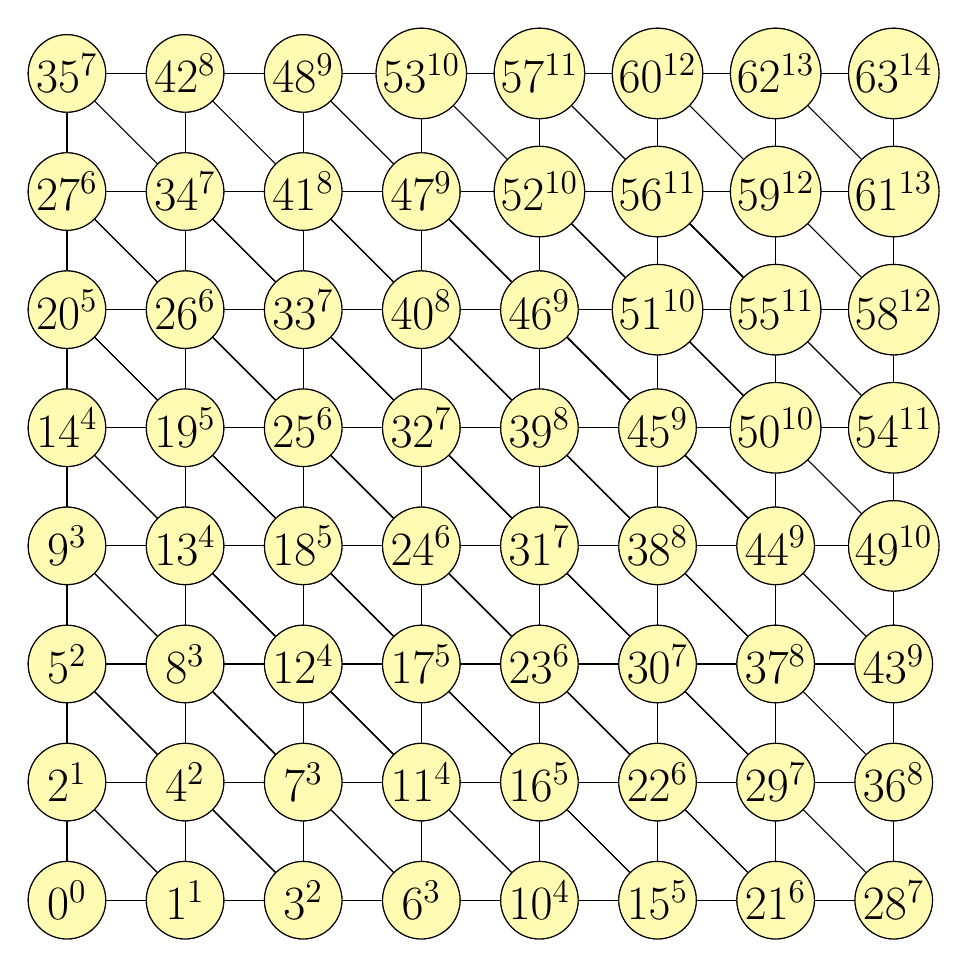
\begin{tikzpicture}[darkstyle/.style={circle,draw,fill=yellow!30!white,minimum size=28, inner sep=0.5pt}]
	\foreach \x in {0,...,7}
	\foreach \y in {0,...,7} 
	{\pgfmathtruncatemacro{\labell}{(\y + \x)*(\y+\x+1)*0.5+\y  }
	\pgfmathtruncatemacro{\labelu}{63 - ((14 - \y - \x)*(14 - \y-\x + 1)*0.5+ 7-\y)  }
	\pgfmathtruncatemacro{\level}{\y + \x  }
	\pgfmathtruncatemacro{\yinv}{7 - \y }
		\node [darkstyle]  (\x\y) at (1.5*\x,1.5*\y) {	\ifthenelse{\x > \yinv} {\LARGE{\labelu$^{\Large{\level}}$}} {\LARGE{\labell$^{\Large{\level}}$}}} ;
		;} 
	
	\foreach \x in {0,...,7}
	\foreach \y [count=\yi] in {0,...,6}  
	{
	\draw (\x\y)--(\x\yi) (\y\x)--(\yi\x) ;
	\draw (\x\y)-- (\y\x);
	}
	
	\foreach \x in {0,...,7}
	\foreach \y in {0,...,7} 
	{\pgfmathtruncatemacro{\labell}{(\y + \x)*(\y+\x+1)*0.5+\y  }
	\pgfmathtruncatemacro{\labelu}{63 - ((14 - \y - \x)*(14 - \y-\x + 1)*0.5+ 7-\y)  }
	\pgfmathtruncatemacro{\level}{\y + \x  }
	\pgfmathtruncatemacro{\yinv}{7 - \y }
	\node [darkstyle]  (\x\y) at (1.5*\x,1.5*\y) {	\ifthenelse{\x > \yinv} {\LARGE{\labelu$^{\Large{\level}}$}} {\LARGE{\labell$^{\Large{\level}}$}}} ;
	;} 
	
%	\draw [white] (0.1,-0.5) rectangle (0.2,-1.5);
	\end{tikzpicture}
\end{document}  